%%%%%%%%%%%%%%%%%%%%%%%%%%%%%%%%%%%%%%%%%
% Journal Article
% LaTeX Template
% Version 1.4 (15/5/16)
%
% This template has been downloaded from:
% http://www.LaTeXTemplates.com
%
% Original author:
% Frits Wenneker (http://www.howtotex.com) with extensive modifications by
% Vel (vel@LaTeXTemplates.com)
%
% License:
% CC BY-NC-SA 3.0 (http://creativecommons.org/licenses/by-nc-sa/3.0/)
%
%%%%%%%%%%%%%%%%%%%%%%%%%%%%%%%%%%%%%%%%%

%----------------------------------------------------------------------------------------
%	PACKAGES AND OTHER DOCUMENT CONFIGURATIONS
%----------------------------------------------------------------------------------------

\documentclass[twoside,twocolumn]{article}

\usepackage{blindtext} % Package to generate dummy text throughout this template 

\usepackage[sc]{mathpazo} % Use the Palatino font
\usepackage[T1]{fontenc} % Use 8-bit encoding that has 256 glyphs
\linespread{1.05} % Line spacing - Palatino needs more space between lines
\usepackage{microtype} % Slightly tweak font spacing for aesthetics

\usepackage[english]{babel} % Language hyphenation and typographical rules

\usepackage[hmarginratio=1:1,top=32mm,columnsep=20pt]{geometry} % Document margins
\usepackage[hang, small,labelfont=bf,up,textfont=it,up]{caption} % Custom captions under/above floats in tables or figures
\usepackage{booktabs} % Horizontal rules in tables

\usepackage{lettrine} % The lettrine is the first enlarged letter at the beginning of the text

\usepackage{enumitem} % Customized lists
\setlist[itemize]{noitemsep} % Make itemize lists more compact

\usepackage{abstract} % Allows abstract customization
\renewcommand{\abstractnamefont}{\normalfont\bfseries} % Set the "Abstract" text to bold
\renewcommand{\abstracttextfont}{\normalfont\small\itshape} % Set the abstract itself to small italic text

\usepackage{titlesec} % Allows customization of titles
\renewcommand\thesection{\Roman{section}} % Roman numerals for the sections
\renewcommand\thesubsection{\roman{subsection}} % roman numerals for subsections
\titleformat{\section}[block]{\large\scshape\centering}{\thesection.}{1em}{} % Change the look of the section titles
\titleformat{\subsection}[block]{\large}{\thesubsection.}{1em}{} % Change the look of the section titles

\usepackage{fancyhdr} % Headers and footers
\pagestyle{fancy} % All pages have headers and footers
\fancyhead{} % Blank out the default header
\fancyfoot{} % Blank out the default footer
\fancyhead[C]{5584F $\bullet$ February 2020 $\bullet$ 4G3} % Custom header text
\fancyfoot[RO,LE]{\thepage} % Custom footer text

\usepackage{titling} % Customizing the title section

\usepackage{hyperref} % For hyperlinks in the PDF

\usepackage{graphicx}
\graphicspath{ {images/} }

\newenvironment{reusefigure}[2][htbp]
  {\addtocounter{figure}{-1}%
   \renewcommand{\theHfigure}{dupe-fig}% If you're using hyperref
   \renewcommand{\thefigure}{\ref{#2}}% Figure counter is \ref
   \renewcommand{\addcontentsline}[3]{}% Avoid placing figure in LoF
   \begin{figure}[#1]}
  {\end{figure}}
\usepackage{wrapfig}
\usepackage{wrapfig}
\usepackage{amsmath}
\usepackage{xcolor}
\usepackage{listings}
\usepackage{subcaption}
\usepackage{pdfpages}
\usepackage{array,multirow,graphicx}
\lstset{
  basicstyle=\ttfamily,
  columns=fullflexible,
  frame=single,
  breaklines=true,
  postbreak=\mbox{\textcolor{red}{$\hookrightarrow$}\space},
}

\newcommand{\threepartdef}[6]
{
	\left\{
		\begin{array}{lll}
			#1 & \mbox{: } #2 \\
			#3 & \mbox{: } #4 \\
			#5 & \mbox{: } #6 \\
			0 & \mbox{: } otherwise
		\end{array}
	\right.
}
%----------------------------------------------------------------------------------------
%	TITLE SECTION
%----------------------------------------------------------------------------------------

\setlength{\droptitle}{-4\baselineskip} % Move the title up

\pretitle{\begin{center}\Huge\bfseries} % Article title formatting
\posttitle{\end{center}} % Article title closing formatting
\title{4G3 - Coursework One -  The asynchronous and irregular state of cortical circuits} % Article title
\author{%
\\
\textsc{Candidate Number: 5584F} \\
}
\date{\today} % Leave empty to omit a date
\renewcommand{\maketitlehookd}{%
\begin{abstract}
\noindent
Leaky integrate and fire neurons were considered in these experiments. Investigations consisted of gradually building up a network starting with a single excitatory input, working up to a randomly connected set of three populations with an external source X, an excitatory E and inhibitory I population. The spike variation of the populations was considered and compared against values within the cortex, the value obtained improved as model complexity grew. It was then shown that the final model had limitations and could be broken by generating a fully connected network.
\newline
\end{abstract}
}

%----------------------------------------------------------------------------------------

\begin{document}
\onecolumn
\includepdf[pages={1}]{Coversheet.pdf}
\twocolumn
\pagenumbering{arabic}
% Print the title
\maketitle
%----------------------------------------------------------------------------------------
%	ARTICLE CONTENTS
%----------------------------------------------------------------------------------------
\section{Introduction}

\lettrine[nindent=0em,lines=3]{M}imicing the architecture of the cortex within a computer has a vast potential for creating complex systems that operate effectively and quickly. Within this report a leaky integrate and fire (LIF) neuron will be investigated and a network built up around it.

%------------------------------------------------

\section{Poisson Spike Train}
An external population 'X' is used to generate N independent spike train inputs to the internal network. These are generated through a Poisson process which can be approximated as a Bernoulli distribution in discrete time when $\delta t$ is sufficiently small  as to ensure a small probability of multiple spikes occurring in one time step. Figure \ref{fig:raster} shows a raster plot for N=1000 over 2 seconds for firing rate $r_x=10Hz$. The theoretic average spike count per neuron is $Tr_x$=20. An average rate of 20.06 was observed.

\begin{figure}[h]
  \centering
    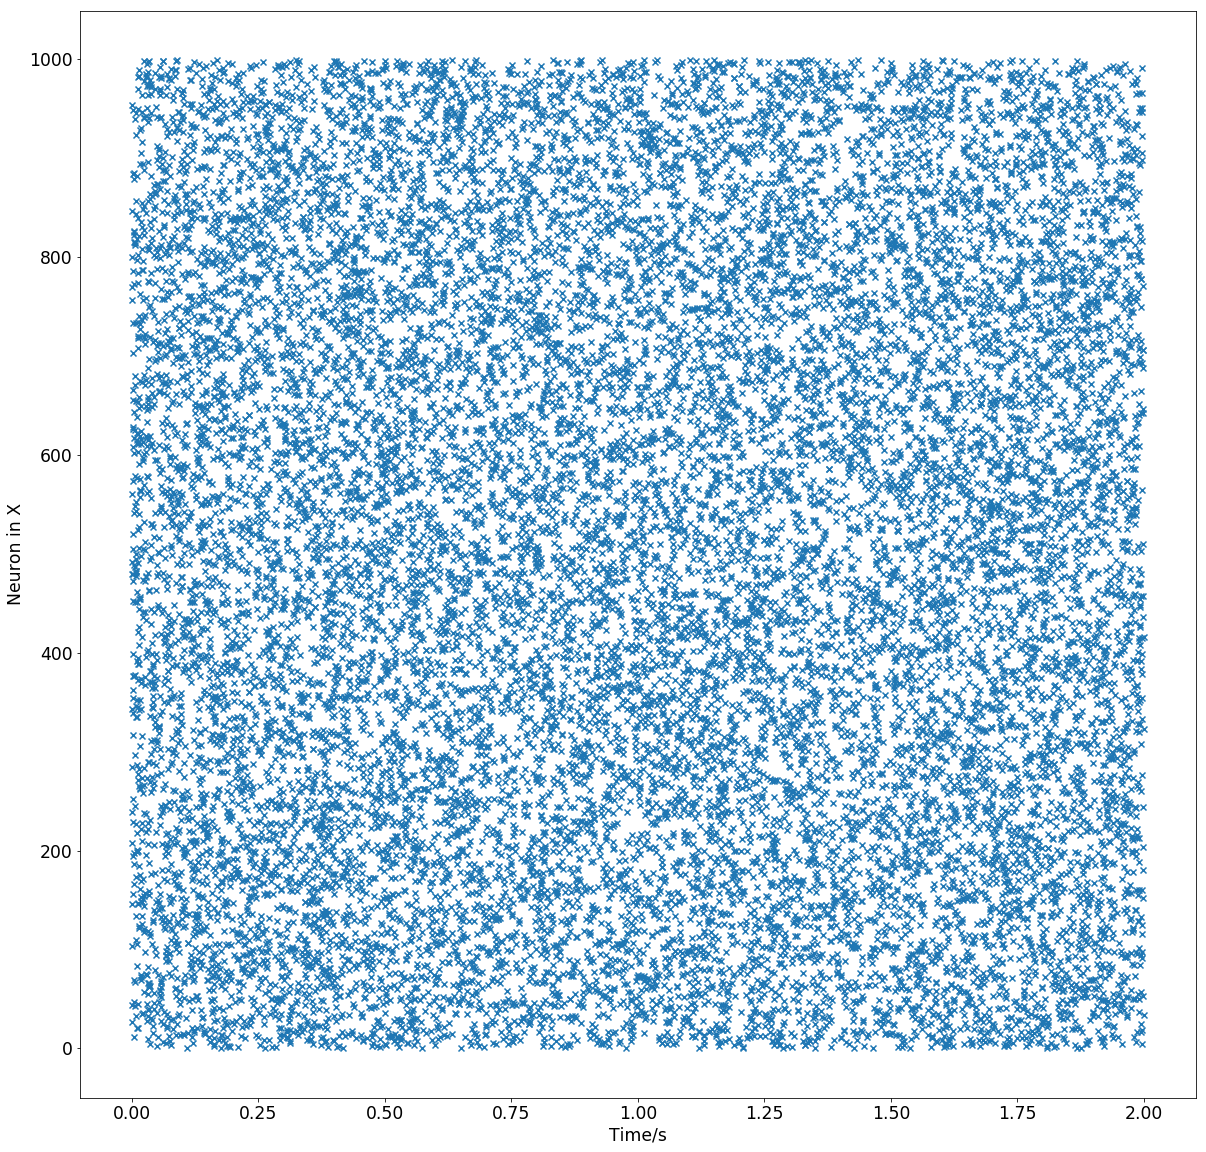
\includegraphics[width=\linewidth]{raster}
  \caption{Raster plot for X population}
  \label{fig:raster}
\end{figure}
 -----------------------------------------------
\section{Single Input LIF Neuron}
These spike trains are inputs to LIF neurons. The membrane potential of these follows equation \ref{eq:LIF} as the population X is excitatory. 

\begin{equation}
V_k = V_{k-1} + \delta t [ \frac{-V_{k-1}}{\tau} + \frac{w}{K} \sum ^K_{j=1} S_j(k-1)]
\label{eq:LIF}
\end{equation}

When the neuron is subject to only one input with w=0.9 the membrane potential and output spike train in figure \ref{fig:2} is observed.

\begin{figure}[h]
  \centering
    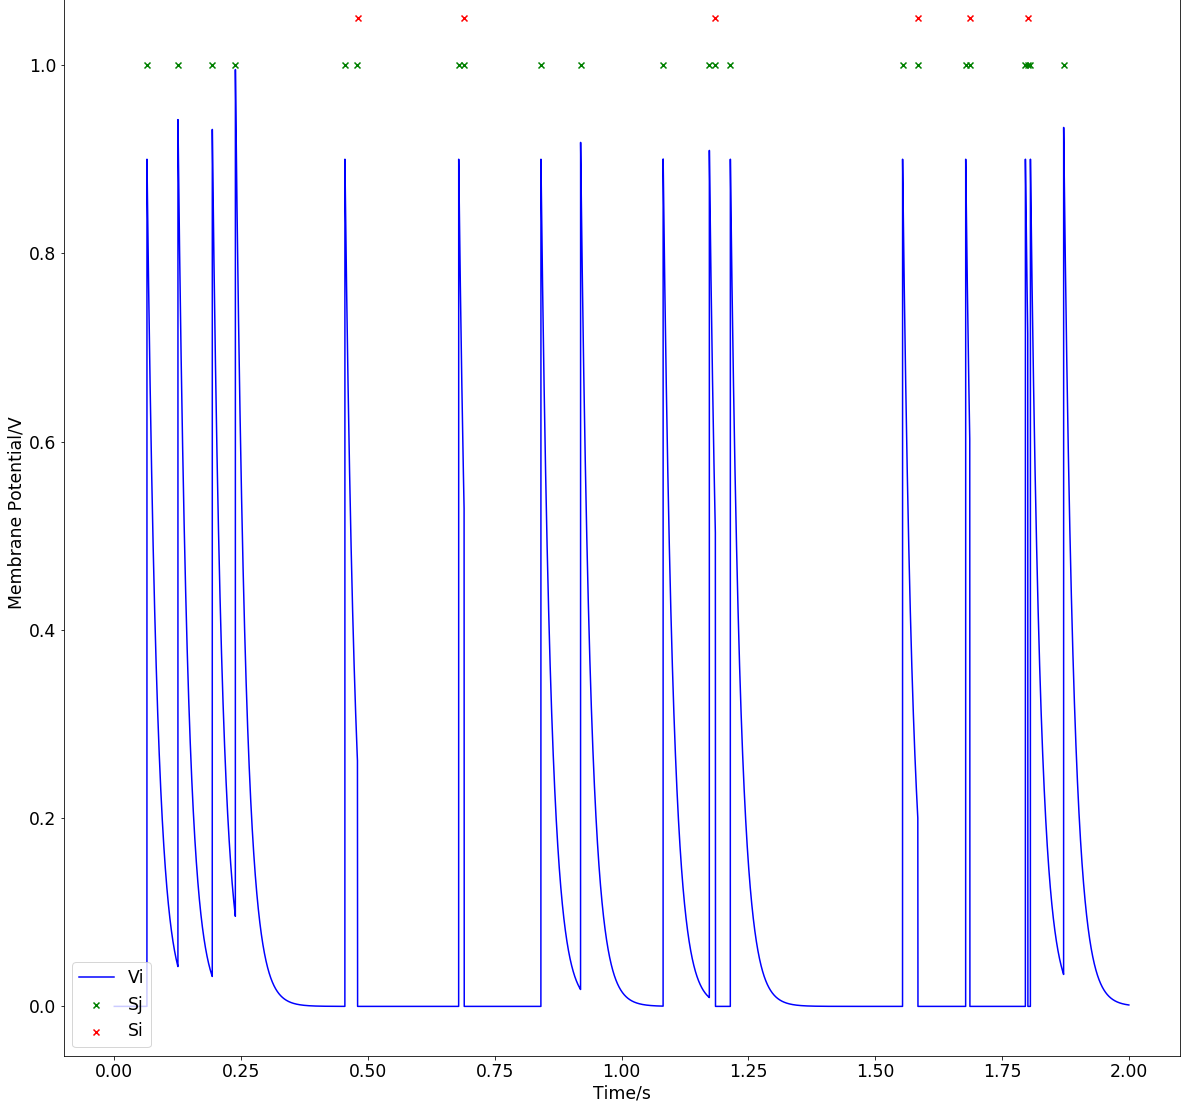
\includegraphics[width=\linewidth]{2}
  \caption{Membrane potential, and output with only a single input}
  \label{fig:2}
\end{figure}
%------------------------------------------------
\section{Multi Input LIF Neuron}
\subsection{a}
A real network consists of each neuron having many inputs. Figure \ref{fig:3a} shows the behaviour of the membrane potential for w=1 with K=100 inputs. The spike and reset mechanism has been disabled to allow the stationary distribution to be observed.

\begin{figure}[h]
  \centering
    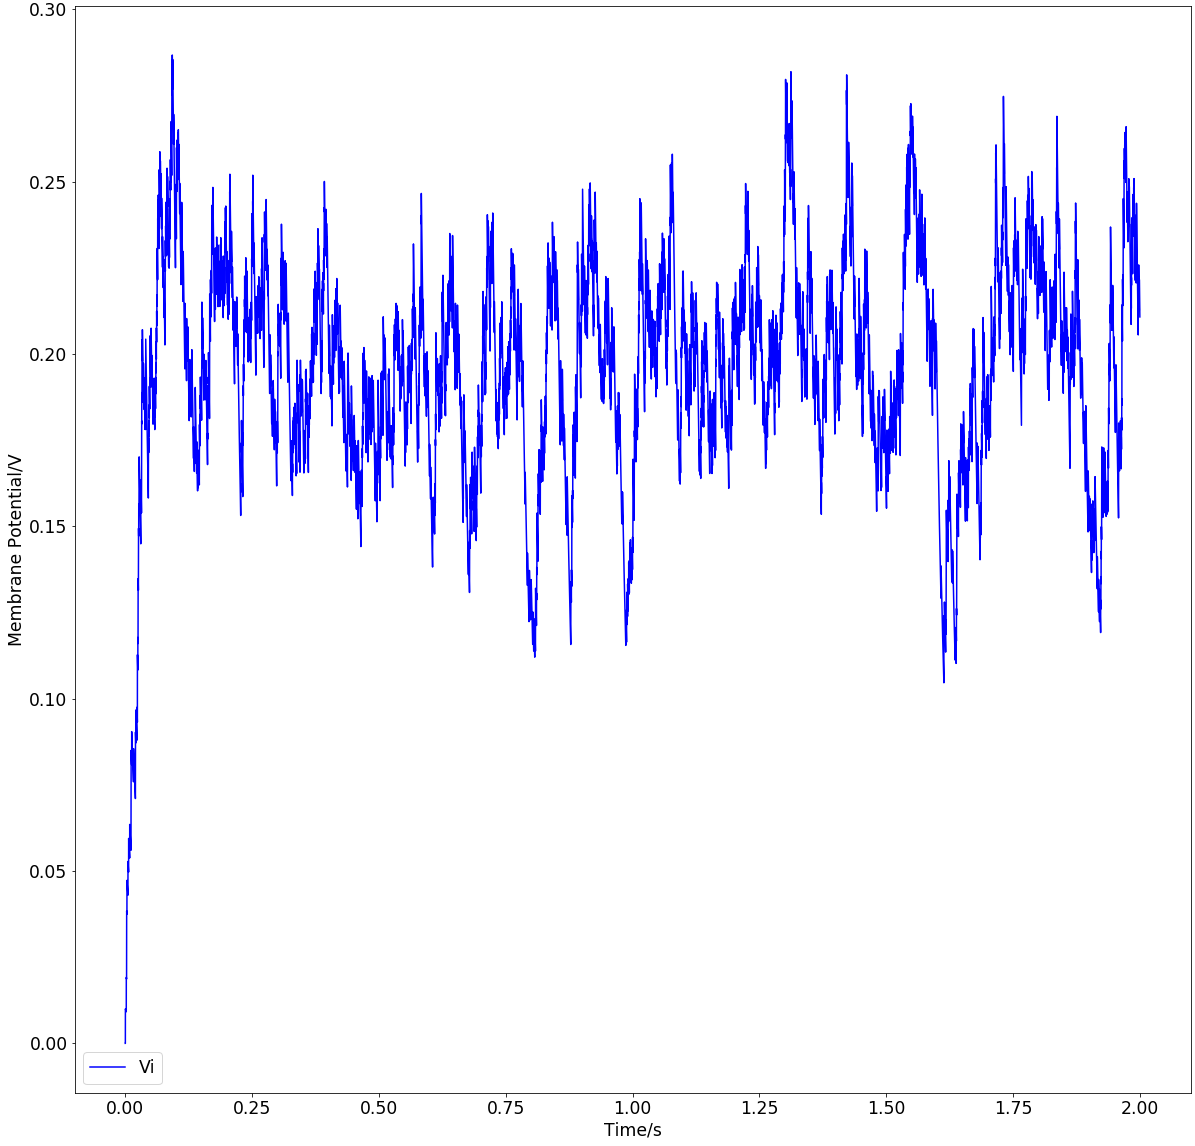
\includegraphics[width=\linewidth]{3a}
  \caption{Multi-Input with potential resetting and w=1}
  \label{fig:3a}
\end{figure}
\subsection{b,c}
After a burn-in time of approximately 100ms the membrane potential reaches a stationary distribution. The theoretical derivation for the mean and variance of V can be seen in the appendix section 1.


Figure \ref{fig:3c} shows the comparison of this theoretical result with values calculated from simulations at varying K values. Showing a good match between simulations and theory.

\begin{figure}[h]
  \centering
    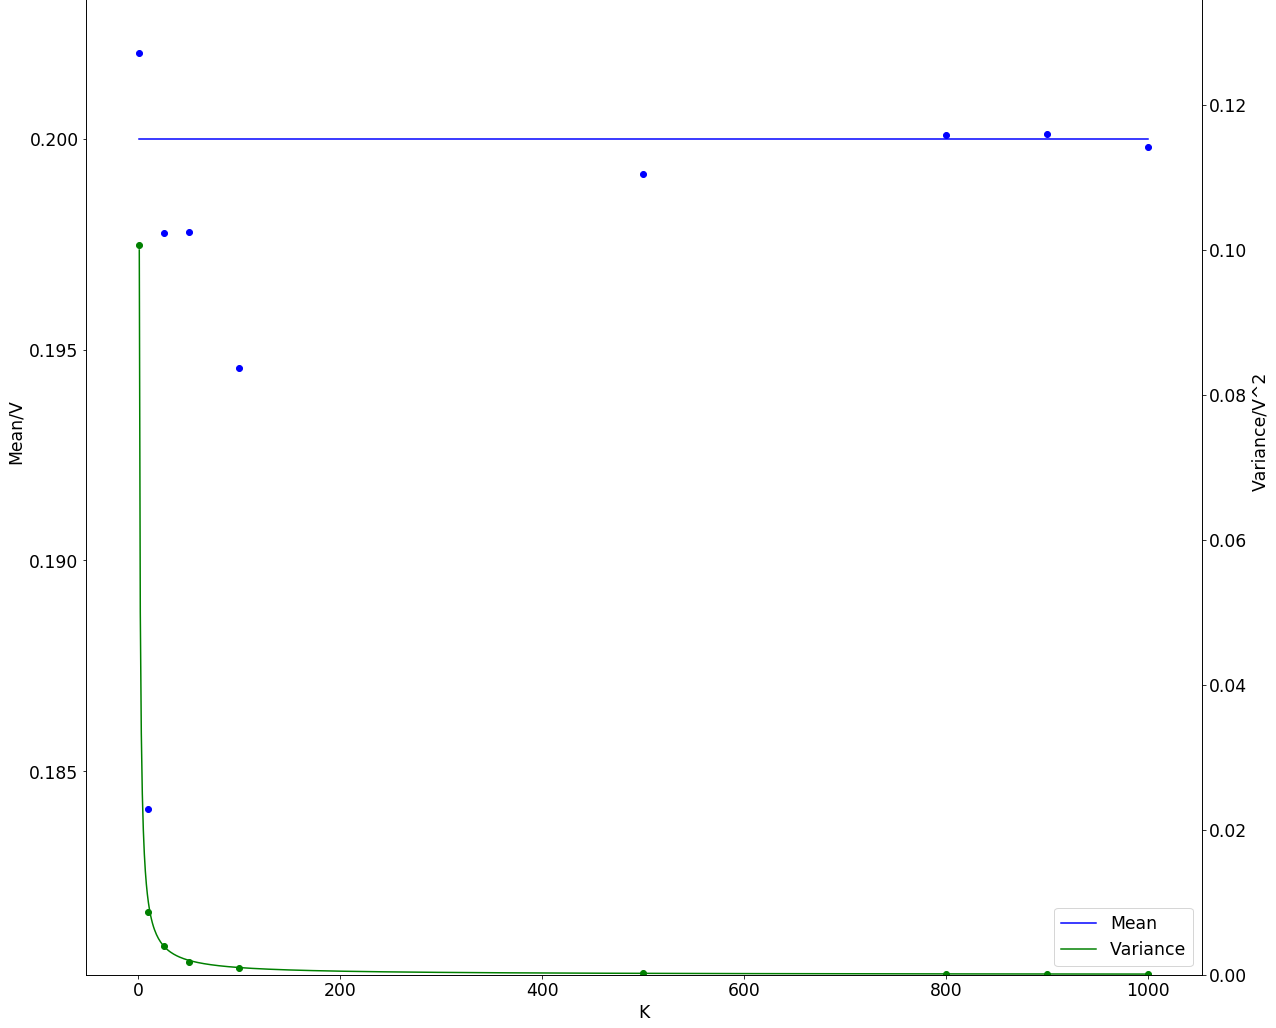
\includegraphics[width=\linewidth]{3c}
  \caption{Membrane potential vs inputs to neuron}
  \label{fig:3c}
\end{figure}

\subsection{d}
As $\mu$ = $wr_x\tau$, the mean can be set to the threshold voltage $V_{th}$ easily by adjusting w. With $V_{th}$=1 a weight of 5 is required. Figure \ref{fig:3d} shows a simulation of this neuron.
\begin{figure}[h]
  \centering
    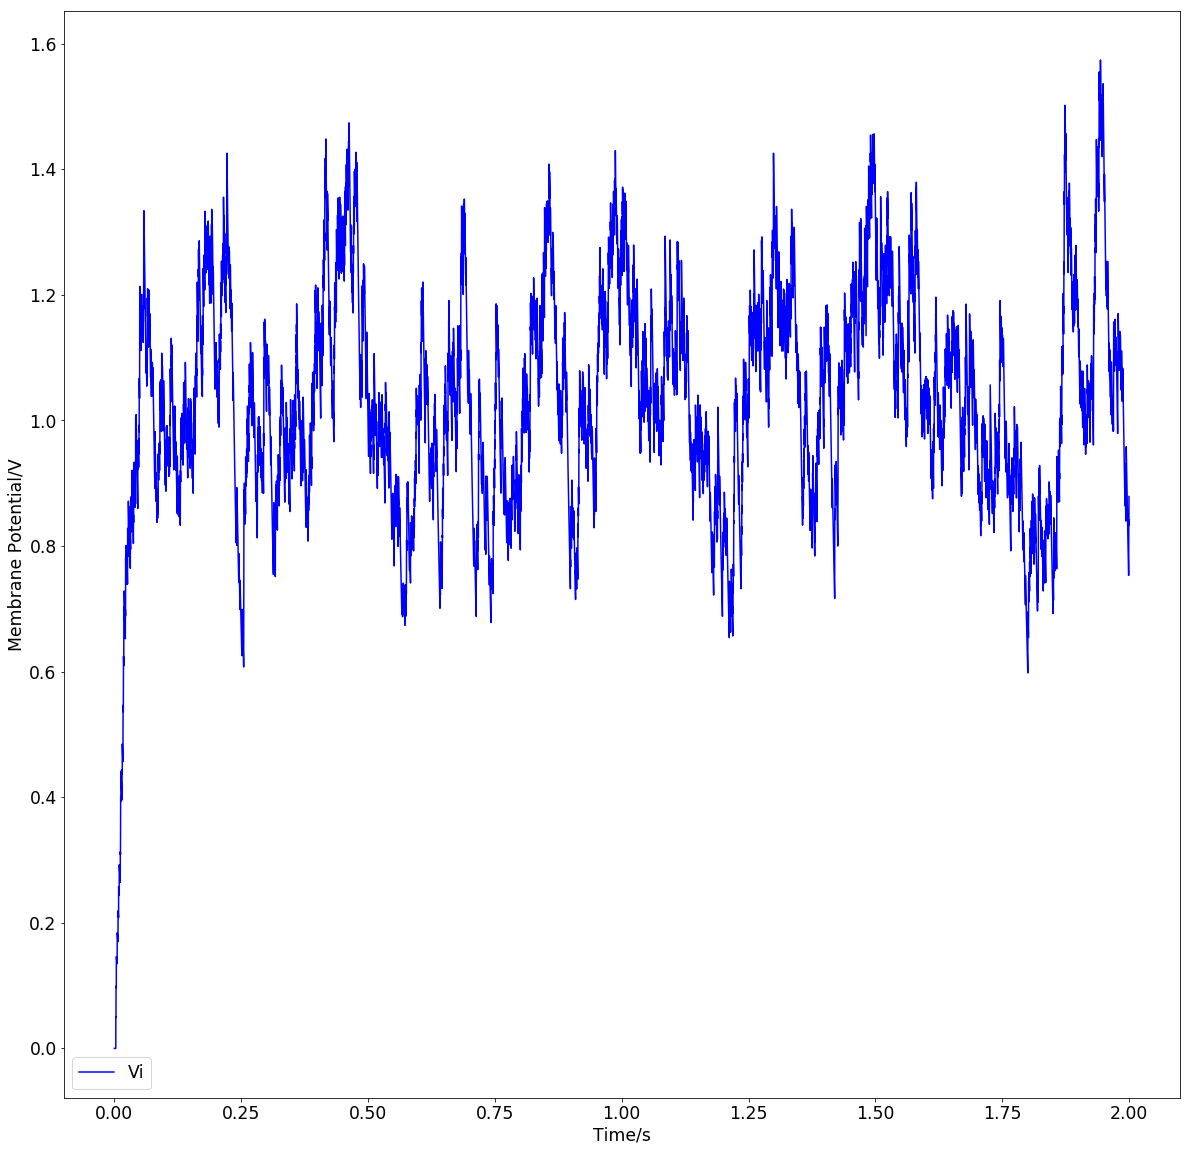
\includegraphics[width=\linewidth]{3d}
  \caption{Mean membrane potential = $V_{th}$=1}
  \label{fig:3d}
\end{figure}


\subsection{e}
The input weight 'w' has a direct effect on neuron firing rate. Table \ref{tab:fr} shows approximate values of w required to achieve a rate of 10Hz. This value varies a lot as it's highly dependant on the random input spike trains from population X. The Fano factor of the output spikes can be computed using the variance and mean spike count within a 100ms window, then dividing the variance by the mean. These factors are also shown in table \ref{tab:fr}. The Fano factor gives information about the spike variability in a network. For our cortex this is greater then 1, which is not what is observed for this simulated network which shows lesser variability. 


\begin{table}[h]
\centering
\begin{tabular}{ c | c | c }
w& r/Hz & Fano factor \\ 
\midrule
4.2&10&0.446 \\
4.22&9& 0.54\\
4.23&10.5&0.5 \\
4.26 & 10.5 &0.487\\
\end{tabular}
\caption{Effect of w on firing rate and Fano factor for a multi input excitatory neuron}
\label{tab:fr}
\end{table}
%------------------------------------------------
\section{Multi E and I Input LIF Neuron}
To Increase variability the model can be extended to take both excitatory inputs which increase potential and inhibitory ones which decrease potential. Equation \ref{eq:LIF} needs to be modified to account for this change. Equation \ref{eq:LIF2} shows the modification required. In these examples the population weights (J) are equal in magnitude (w) but of opposite sign.

\begin{equation}
V_k = V_{k-1} + \delta t [  \frac{-V_{k-1}}{\tau} + \sum _{\beta \in [E,I,X] } \frac{J_{\alpha \beta}}{\sqrt{K}} \sum ^K_{j=1} S_j(k-1)]
\label{eq:LIF2}
\end{equation}
\subsection{a}
The theoretic mean and variance of V can once again be calculated. This follows the same method as in appendix section 1. The variance and mean of h(k) is $2w^2r_x(\frac{1}{\delta t} -r_x)$ and 0 respectively. These can then be used as before once again ignoring terms of $\mathbb{O}(\delta t^2$).
The mean of V is then calculated to be 0, and the variance is constant with K and is $\tau w^2 r_x$.
\subsection{b}
The effect of w on firing rate and spike variability can be estimated with the new model. Table \ref{tab:fr2} shows the values of w that achieve a rate of approximately 10Hz. The Fano factor observed is closer to or above 1 and therefore closer to the variability of spikes in the cortex and shows the model has improved with the addition on I inputs. However, as the Fano factor sometimes is below 1 there are other improvements that may make the model more realistic.

\begin{table}[h]
\centering
\begin{tabular}{ c | c | c }
w& r/Hz & Fano factor \\ 
\midrule
1.44&10&1.06 \\
1.46&10.5&1.34\\
1.48&9.5& 0.63\\

\end{tabular}
\caption{Effect of w on firing rate and Fano factor for a multi E/I input neuron}
\label{tab:fr2}
\end{table}
%------------------------------------------------------
\section{Full Network}
The next step in making a full network is to set up each neuron in E and I so that it takes K random inputs from each of the E,I,X populations to form the network shown in figure \ref{fig:net}. The connectivity weights will take the values $J_{EE}=1$, $J_{IE}=1$, $J_{EI}=-2$, $J_{II}=-1.8$, $J_{EX}=1$, $J_{IX}=0.8$.

\begin{figure}[h]
  \centering
    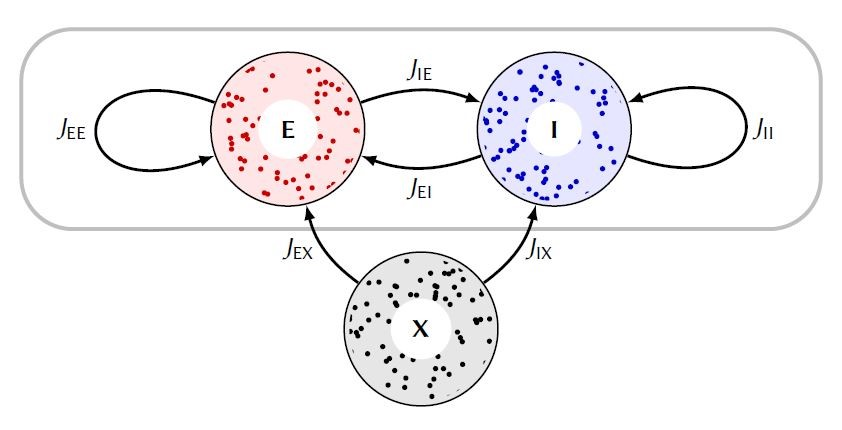
\includegraphics[width=\linewidth]{network}
  \caption{Full Network}
  \label{fig:net}
\end{figure}
\begin{figure}[h]
  \centering
  \begin{subfigure}[t]{0.4\textwidth}
    \includegraphics[width=\linewidth]{e}
  \caption{E} 
  \label{sub:E}
  \end{subfigure}
  \begin{subfigure}[t]{0.4\textwidth}
    \includegraphics[width=\linewidth]{i}
  \caption{I}
  \label{sub:I}
  \end{subfigure}
  \caption{Full network simulation for one neuron in E and I}
  \label{fig:fn}
\end{figure}
\subsection{a}
The mean firing rate of population E and I can be calculated as follows:

\begin{gather}
\begin{bmatrix}
J_{EE} & J_{EI}  \\
J_{IE} & J_{II}  \\
\end{bmatrix}
\begin{bmatrix}
r_E  \\
r_I \\
\end{bmatrix}
=
-\begin{bmatrix}
J_{EX}  \\
J_{IX} \\
\end{bmatrix}r_x
+ \mathbb{O}(\frac{1}{\sqrt{K}}) \nonumber 
\end{gather}

With the values previously stated and the constant taken to be $\frac{1}{\sqrt{K}}=0.1$ results in $r_E,r_I$ = $1.1r_x, r_x$ respectively after solving the linear equations. With sufficiently large K $r_x=r_E=r_I$.




\subsection{b,c}
With N=1000, and K=100 the network was simulated for 2 seconds for varies values of $r_x$. Table \ref{tab:r} shows the simulated rates for population E and I. Both rates are always higher then $r_x$ with the rate of E neurons being the highest. The ordering agrees with the previous predictions. However, the simulated results show a relationship of approximately $r_E,r_I$ = $1.25r_x, 1.13r_x$. This difference is likely due to the network (K,N) being small and creating loops within the network that increase the firing rate. In the cortex (K,N) is large enough that this is less likely.

\begin{table}[h]
\centering
\begin{tabular}{ c | c | c }
$r_x$& $<r_E>$ & $<r_I>$ \\ 
\midrule
5&6.95&5.83 \\
10&12.97& 11.64\\
15&18.29&16.88 \\
20&24.20&22.51\\
\end{tabular}
\caption{Average firing rate of E/I neurons given an input of rate $r_x$}
\label{tab:r}
\end{table}

Figure \ref{fig:fn} shows an example neuron in E and I behaving as expected.



\subsection{d}
Reducing the network to N=K=100 causes the average rates to be $r_E$=40, $r_I$=20. Figure \ref{fig:nk} shows the membrane potential of every E and I neuron. As each neuron is connected to every other neuron each neuron will have the same connections causing the behaviour of a population to be identical.  This is shown in the figure as the lines all overlap, meaning a population will behave identically as inputs, weights and connections are the same. There are differences between the two populations as the connectivity weights differ slightly, causing the difference in behaviour at the spikes. The E population fires twice as often as the I population. Upon closer examination this occurs because E neurons fire first, the next timestep they'll fire again in addition to the I population firing. This happens because all E neurons are inputs back into their population so upon all firing the potential of the E population can be raised above the threshold again within one timestep, ( $\frac{K}{\delta t}\frac{J_{EE}}{\sqrt{K}} >V_{th}$). This double fire doesn't occur when the I population fires as the inhibitory connection lowers the potentials. If $J_{EX}$ and $J_{IX}$ are reversed then the firing rates become roughly 0 and 17 for the E,I populations. This is because with a greater weight to I from X the I population will always fire first, causing the E population lose potential. This is shown in figure\ref{fig:5d}.
\newline
Several assumptions which may have been broken include. Random network connectivity broken as all connections identical. K=N which may cause chaotic behaviour as an eigenvalue value could equal 1. Loops within the network have additional side effects that weren't considered.
\begin{figure}[h]
  \centering
    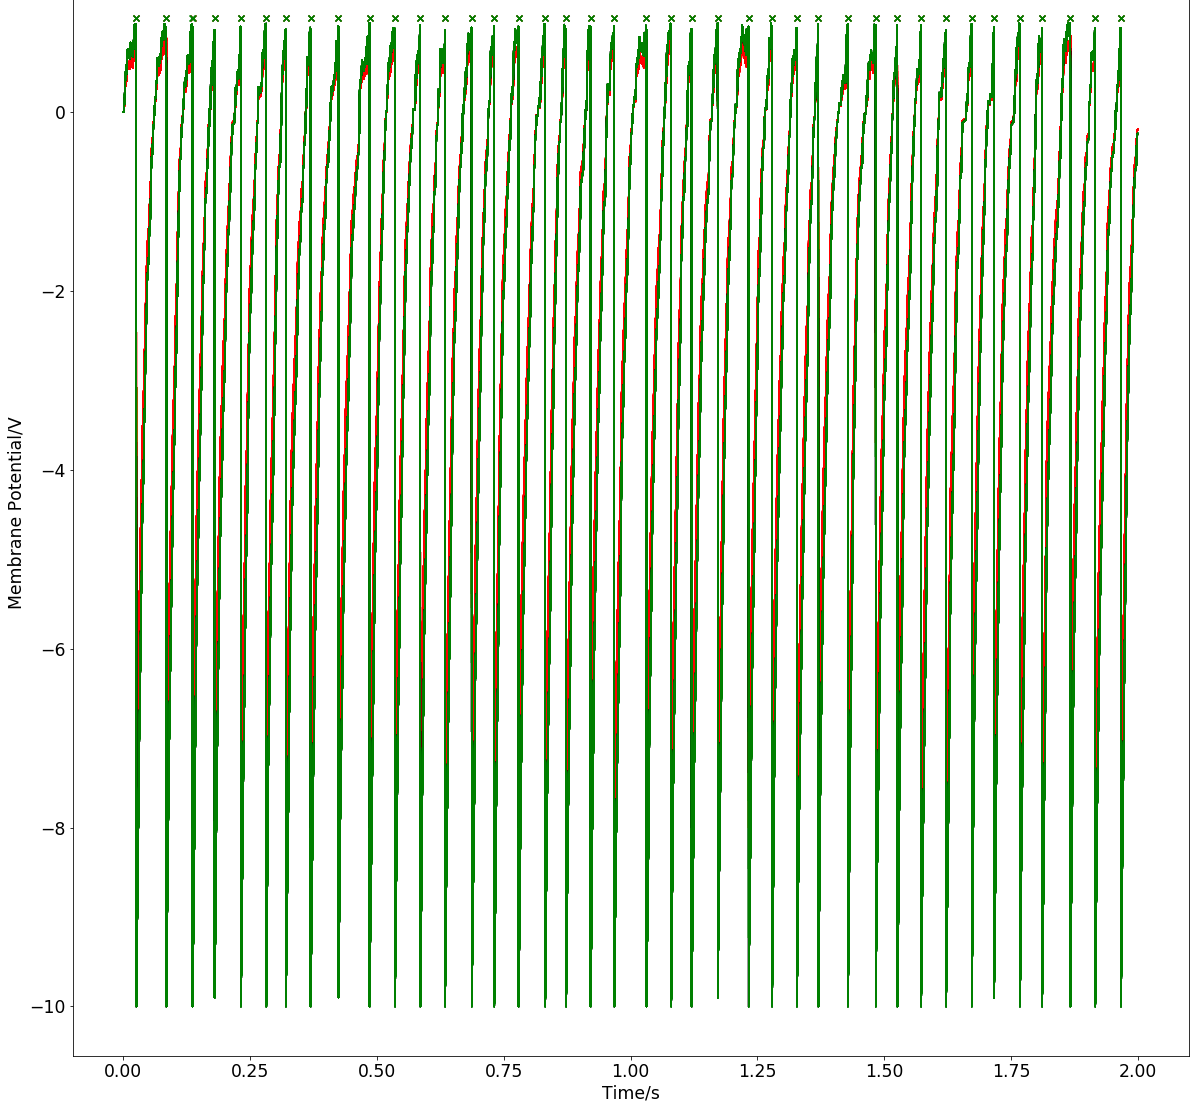
\includegraphics[width=\linewidth]{k=n}
  \caption{Full Network when K=N=100, showing all neuron activity with I in red and E in green}
  \label{fig:nk}
\end{figure}

\begin{figure}[h]
  \centering
    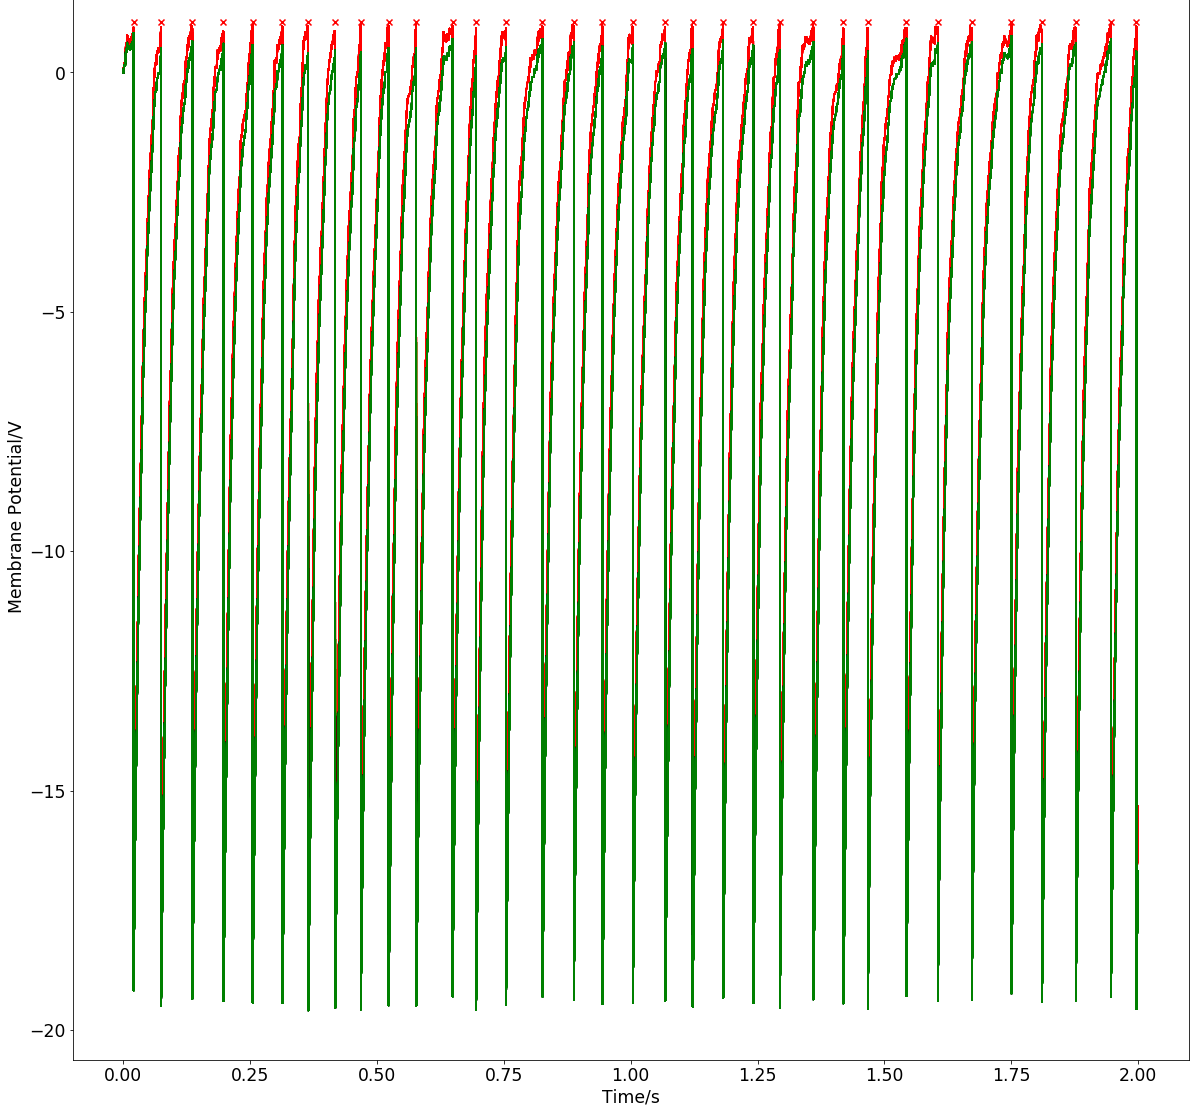
\includegraphics[width=\linewidth]{5d}
  \caption{Full Network when K=N=100, showing all neuron activity with I in red and E in green, with $J_{EX}$ and $J_{IX}$ reversed}
  \label{fig:5d}
\end{figure}
%------------------------------------------------

%----------------------------------------------------------------------------------------
\onecolumn
\section{Appendix}

\subsection{1. Derivation of mean and variance of V(t)}
First consider the spike train $S_j$:
\begin{gather}
S_j(k) \sim \mathbb{B}(r_x\delta t) \nonumber \\
<S_j(k)> = r_x \nonumber \\
<<S_j(k)>> = \mathbb{E}(S_j(k)^2) - \mu^2 \nonumber\\
= \frac{r_x\delta t}{\delta t^2} + 0 -r_x^2 = r_x(\frac{1}{\delta t} - r_x)\nonumber\\
\end{gather}
Taking note that each input neuron j is independent and uncorrelated allows the following manipulation to occur for calculating the moments of h(k). This is because $Cov[S_i(k)S_j(k)]$=0 for $i\neq j$, allowing the variance of a sum to equal the sum of variances.
\begin{gather}
h(k) = \frac{w}{K}\sum_{j=1}^KS_j(k)\nonumber\\
<h(k)> =\frac{w}{K}\sum_{j=1}^K \mathbb{E}[S_j(k)] = \frac{w}{K} Kr_x = wr_x \nonumber\\
<<h(k)>> = \frac{w^2}{K^2}   \sum_{j=1}^K  <<S_j(k)>>\nonumber \\
= \frac{w}{K}^2   K  r_x(\frac{1}{\delta t} - r_x)  = \frac{w^2r_x}{K} (\frac{1}{\delta t} - r_x)\nonumber\\
\end{gather}
Using equation \ref{eq:LIF} and taking advantage that when stationary the moments of V and h are equal at times k and k-1, the following simplifications can occur:
\begin{gather}
<V_k> = <V_{k-1}> + \delta t [ \frac{-<V_{k-1}>}{\tau} + <h_{k-1}>]\nonumber\\
<V_{\infty}> = <V_{\infty}> + \delta t [ \frac{-<V_{\infty}>}{\tau} + <h_{\infty}>]\nonumber\\
<V_{\infty}> = \tau <h_{\infty}> = \tau wr_x \nonumber\\ 
\nonumber\\
<<V_k>> =(1-\frac{\delta t }{\tau})^2 <<V_{k-1}>> + \delta t^2<<h_{k-1}>>\nonumber\\
<<V_{\infty}>> =(1-\frac{\delta t }{\tau})^2 <<V_{\infty}>> + \delta t^2<<h_{\infty}>>\nonumber\\
<<V_{\infty}>>(1-(1-\frac{\delta t }{\tau})^2) = \delta t^2 <<h_{\infty}>> = \delta t^2(\frac{w^2r_x}{K} (\frac{1}{\delta t} - r_x) ) \nonumber\\
<<V_{\infty}>>(\frac{2\delta t}{\tau} - \frac{\delta t^2}{\tau^2}) = \delta t\frac{w^2r_x}{K} + \delta t^2 \frac{w^2r_x^2}{K}\nonumber \\
\end{gather}
Eliminating everything of $\mathbb{O}(\delta t^2)$ results in the following:
\begin{gather}
<<V_{\infty}>>\frac{2\delta t}{\tau} = \delta t\frac{w^2r_x}{K}\nonumber \\
<<V_{\infty}>> = \frac{w^2r_x\tau}{2K} \nonumber \\
\end{gather}

%------------------------------------------------
\end{document}
